\documentclass{beamer} %

%%%BASICS
\usepackage[utf8]{inputenc}
\usepackage{csquotes}

%%%START THEME SETTINGS
\usetheme{Madrid}
% \usecolortheme{beaver}
\useoutertheme{infolines}  % Subsection information on top of the slide
\usefonttheme{professionalfonts}

% \setbeamercolor{item projected}{bg=red!80!black} %<---- color of ball
% \setbeamercolor{enumerate subitem}{fg=red!80!black} %<--- color of number % 
% in second level

%%%END THEME SETTINGS

%%%START APA
\usepackage[british]{babel}

\usepackage{datetime}  % Inserting dates
\usepackage{graphicx}  % Lets you insertPDF images
\usepackage{subcaption}  % Multiple captions of images

% ____ Bibliography ____
\usepackage{natbib} %Bibliography.
% \setcitestyle{numbers} %Cite as numbers or author-year.
\bibliographystyle{plain} %Reference style.
% ______________________

% Confusion Matrix
\usepackage{array}
\usepackage{multirow}
\newcommand\MyBox[2]{
  \fbox{\lower0.75cm
    \vbox to 1.7cm{\vfil
      \hbox to 1.7cm{\centering \hfil\parbox{0.5cm}{#1\\#2}\hfil}
      \vfil}%
  }%
}

% Tables
\usepackage{array}
\newcolumntype{C}[1]{>{\centering\arraybackslash}m{#1}}

%% APA citing
%% \cite{t} - Uthor und Richter, 2010
%% \textcite{t} - Uthor und Riter (2010)
%% \parencite{t} - (Uthor & Riter, 2010)
%% \parencite[Chapt.~4]{t} - (Uthor & Riter, 2010, S. 15)
%%%END APA

\newcommand{\homeCOne}{../../Chapter 1 - Metalabeling/Draft}
\newcommand{\homeCTwo}{../../Chapter 2 - FracDiff/Draft}
\newcommand{\home}{../Draft}

\title[Exploring ML Advances in Finance]
{Exploring Machine Learning Advances in Finance}
\author[GCB]{Guillermo Creus Botella}
\newdate{date}{12}{1}{2021}
\titlegraphic{
	\begin{figure}
		\centering
		\begin{minipage}{.5\textwidth}
			\centering
			\includegraphics[width=.8\textwidth]{"\home/img/logo_UPC"}
		\end{minipage}%
		\begin{minipage}{.5\textwidth}
			\centering
			\includegraphics[width=.8\textwidth]{"\home/img/logo_HKUST"}
		\end{minipage}
	\end{figure}	
}
\date{\displaydate{date}}

\AtBeginSection[]{
  \begin{frame}
  \vfill
  \centering
  \begin{beamercolorbox}[sep=8pt,center,shadow=true,rounded=true]{title}
    \usebeamerfont{title}\insertsectionhead\par%
  \end{beamercolorbox}
  \vfill
  \end{frame}
}

\begin{document}
\begin{frame}
	\maketitle
\end{frame}

\begin{frame}{Contents}
	\tableofcontents
\end{frame}

\section{Primer in financial data}
\begin{frame}{Asset log-prices}
	\begin{itemize}
		\item Let $p_t$ be the price of an asset at (discrete) time index $t$
		
		\item For modeling purposes, the natural logarithm of prices will be 
		used $y_t = \log (p_t)$ (log-prices)
	\end{itemize}
	
	\begin{figure}
		\centering
		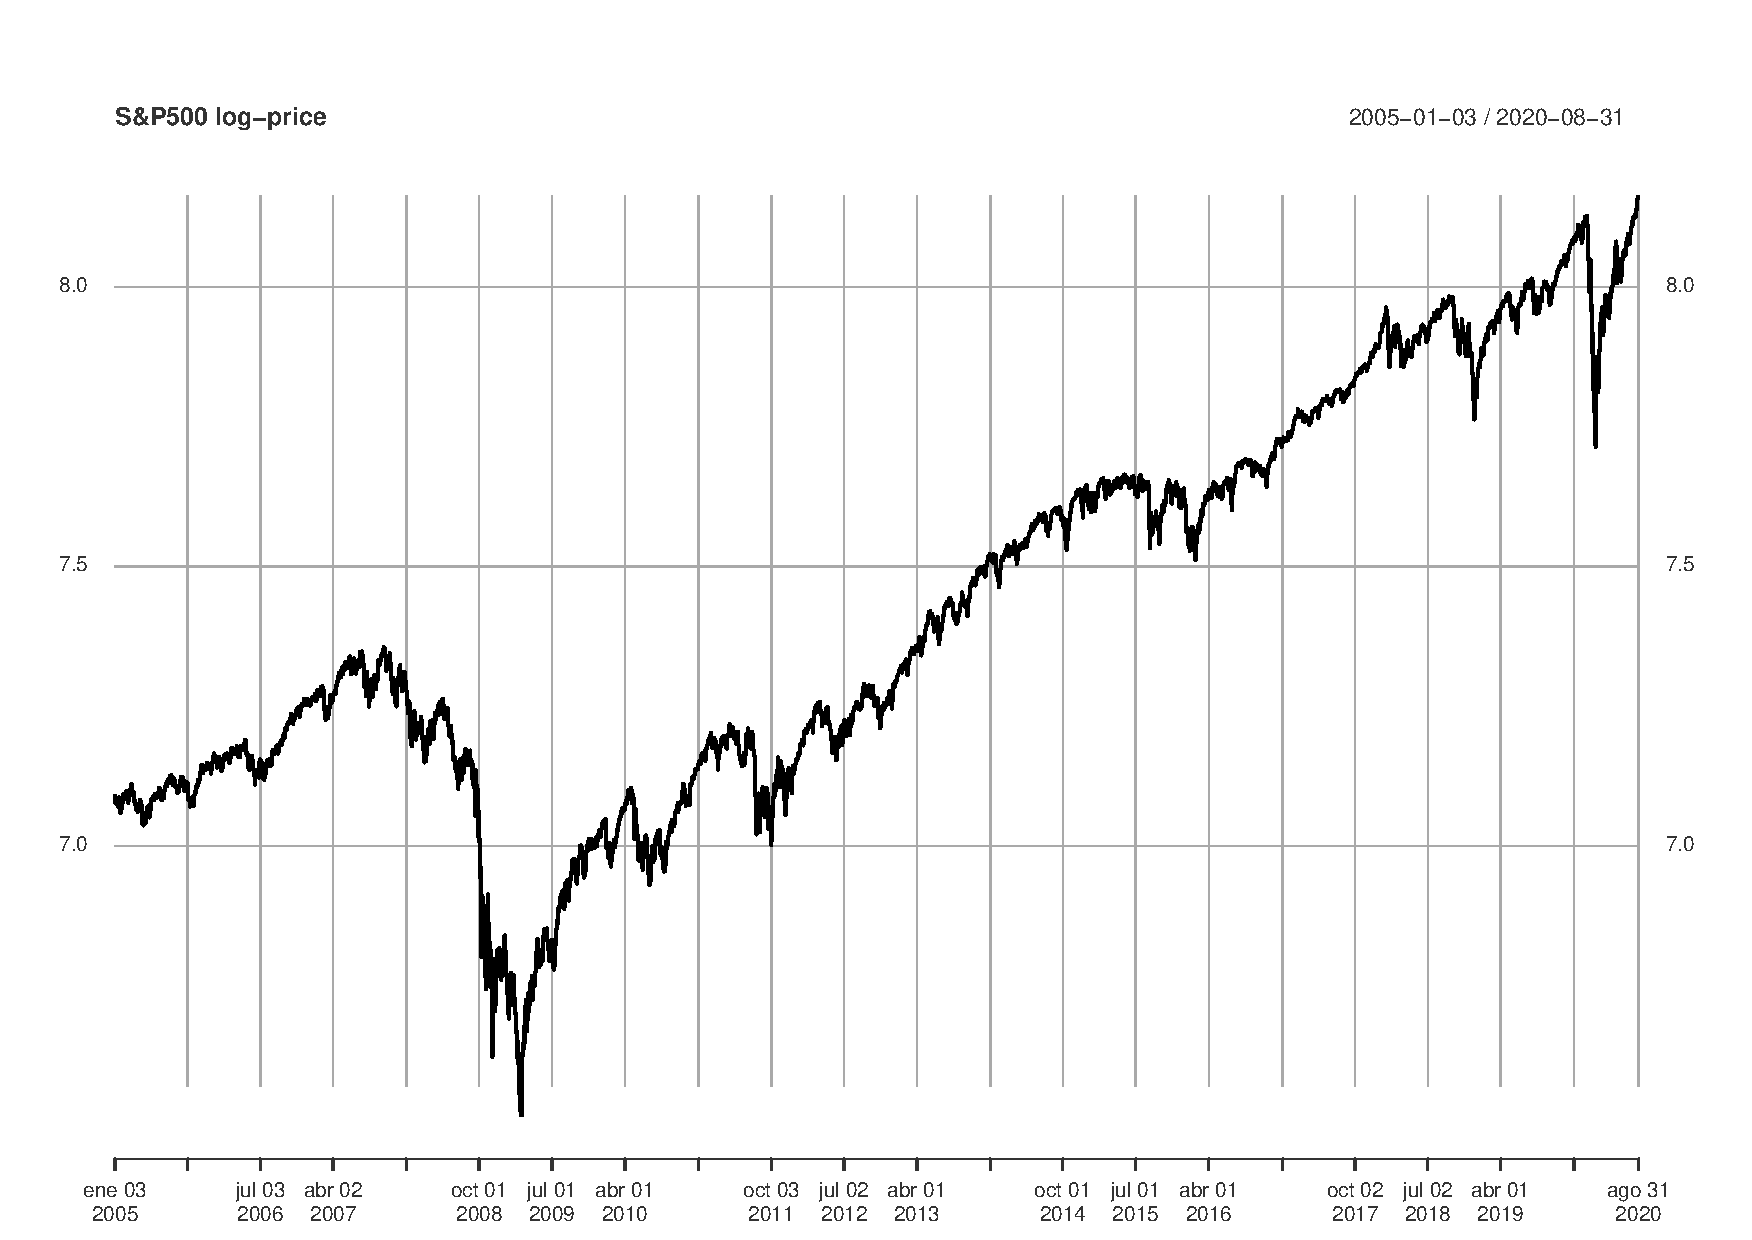
\includegraphics[scale=.25]{img/SP500}
		\caption{S\&P 500 log-prices}
	\end{figure}
\end{frame}

\begin{frame}{Asset returns \& volatility}
	\begin{itemize}
		\item \textbf{Linear returns:} $R_t = \frac{p_t - p_{t-1}}{p_{t-1}} = 
		\frac{p_t}{p_{t-1}} - 1$
		
		\item \textbf{Log-returns:} $r_t = \log \left( \frac{p_t}{p_{t-1}} 
		\right) = y_t - y_{t-1}$
	\end{itemize}

	\vspace{.2cm}	
	
	Note that $r_t = \log (1+R_t)$ and $r_t \approx R_t$ whenever $R_t 
	\approx 0$
	
	\vspace{.2cm}
	
	\begin{itemize}
		\item \textbf{Volatility:} Measures the variation of returns $\sigma 
		= \sqrt{\text{Var}[r_t]}$
	\end{itemize}
	
	\begin{figure}
		\centering
		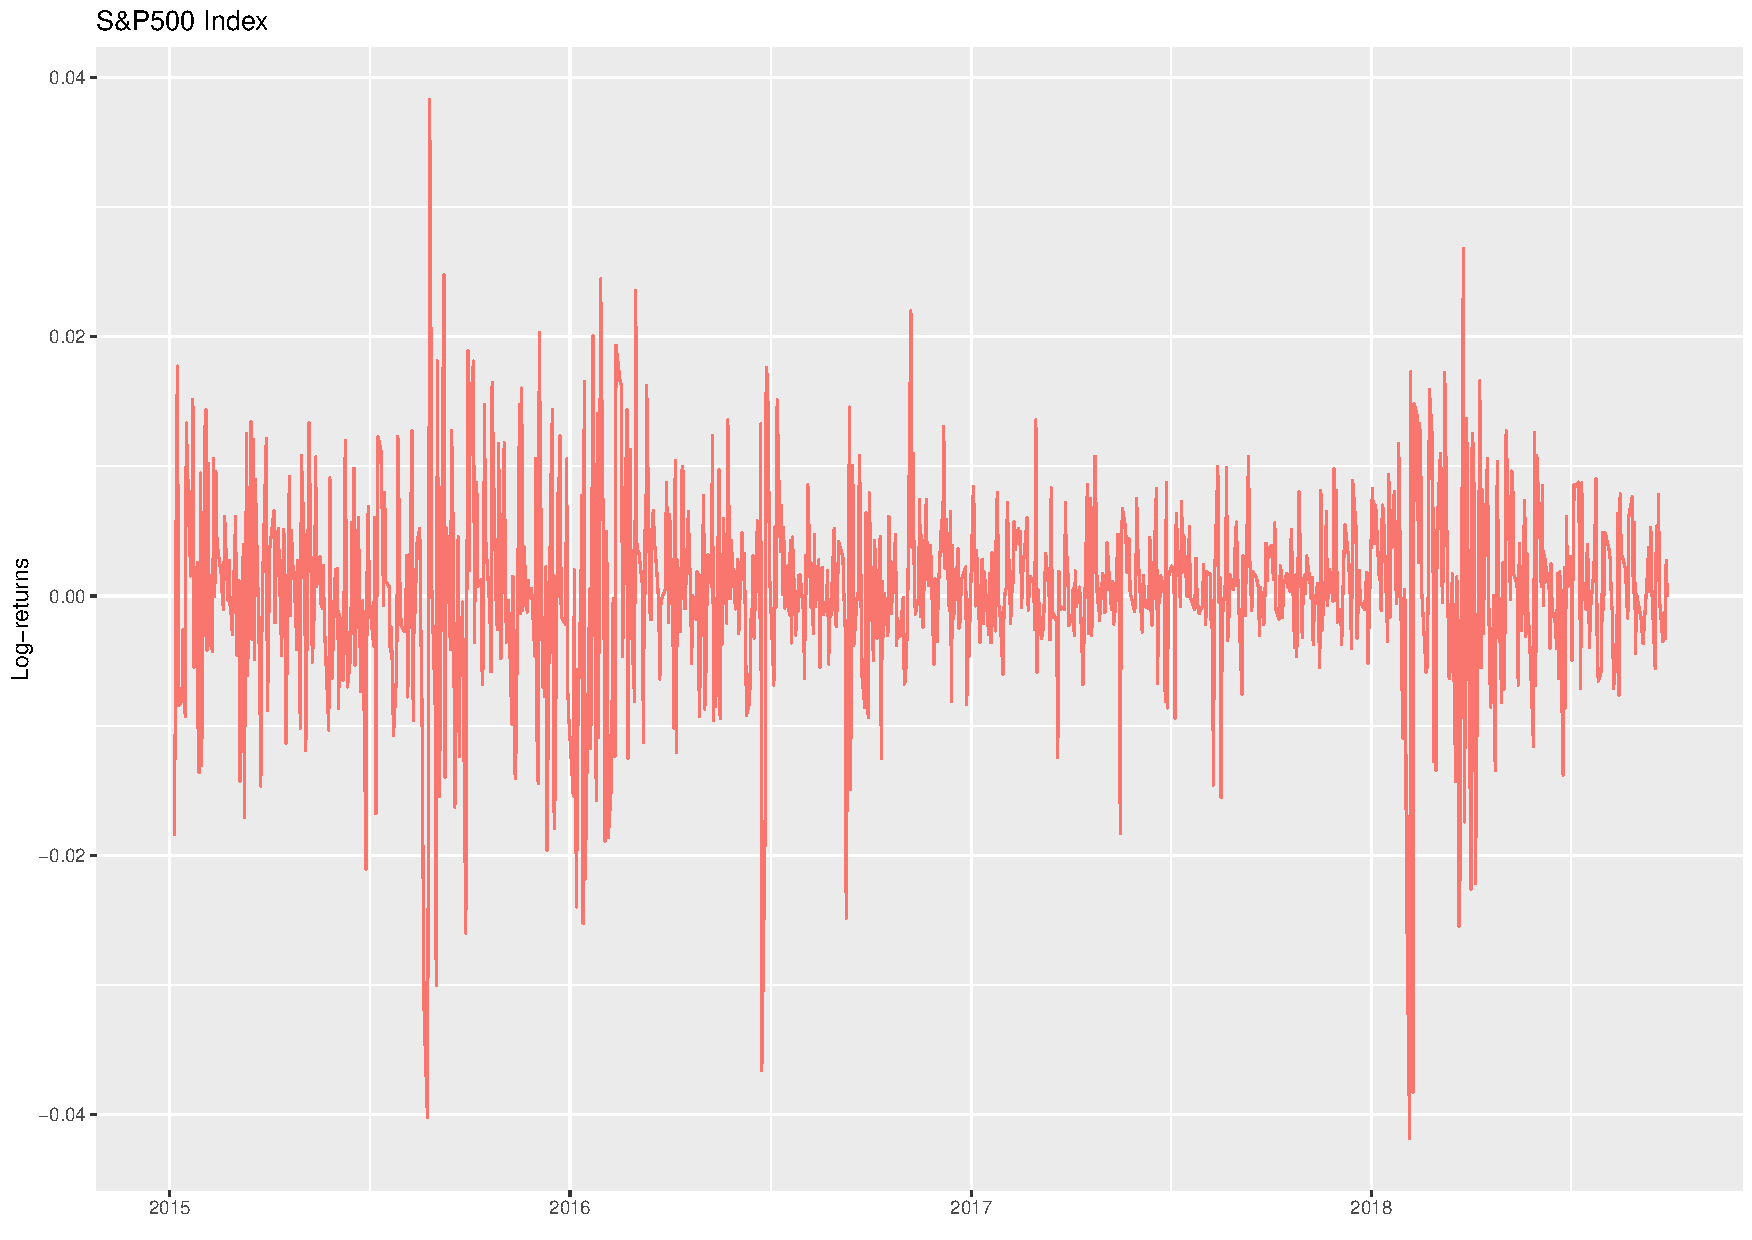
\includegraphics[scale=.2]{../Draft/img/finData/logReturns}
		\caption{S\&P 500 log-returns}
	\end{figure}
\end{frame}

\begin{frame}{Stylized facts}
	\begin{center}
		\begin{enumerate}
			\item Absence of autocorrelations
			\item Heavy tails
			\item Gain/loss asymmetry
			\item Aggregational Gaussianity
			\item Intermittency
			\item Volatility clustering
		\end{enumerate}
	\end{center}

\end{frame}

\begin{frame}{Stylized facts}

	\begin{columns}
		\begin{column}{.5\textwidth}
			\begin{figure}
				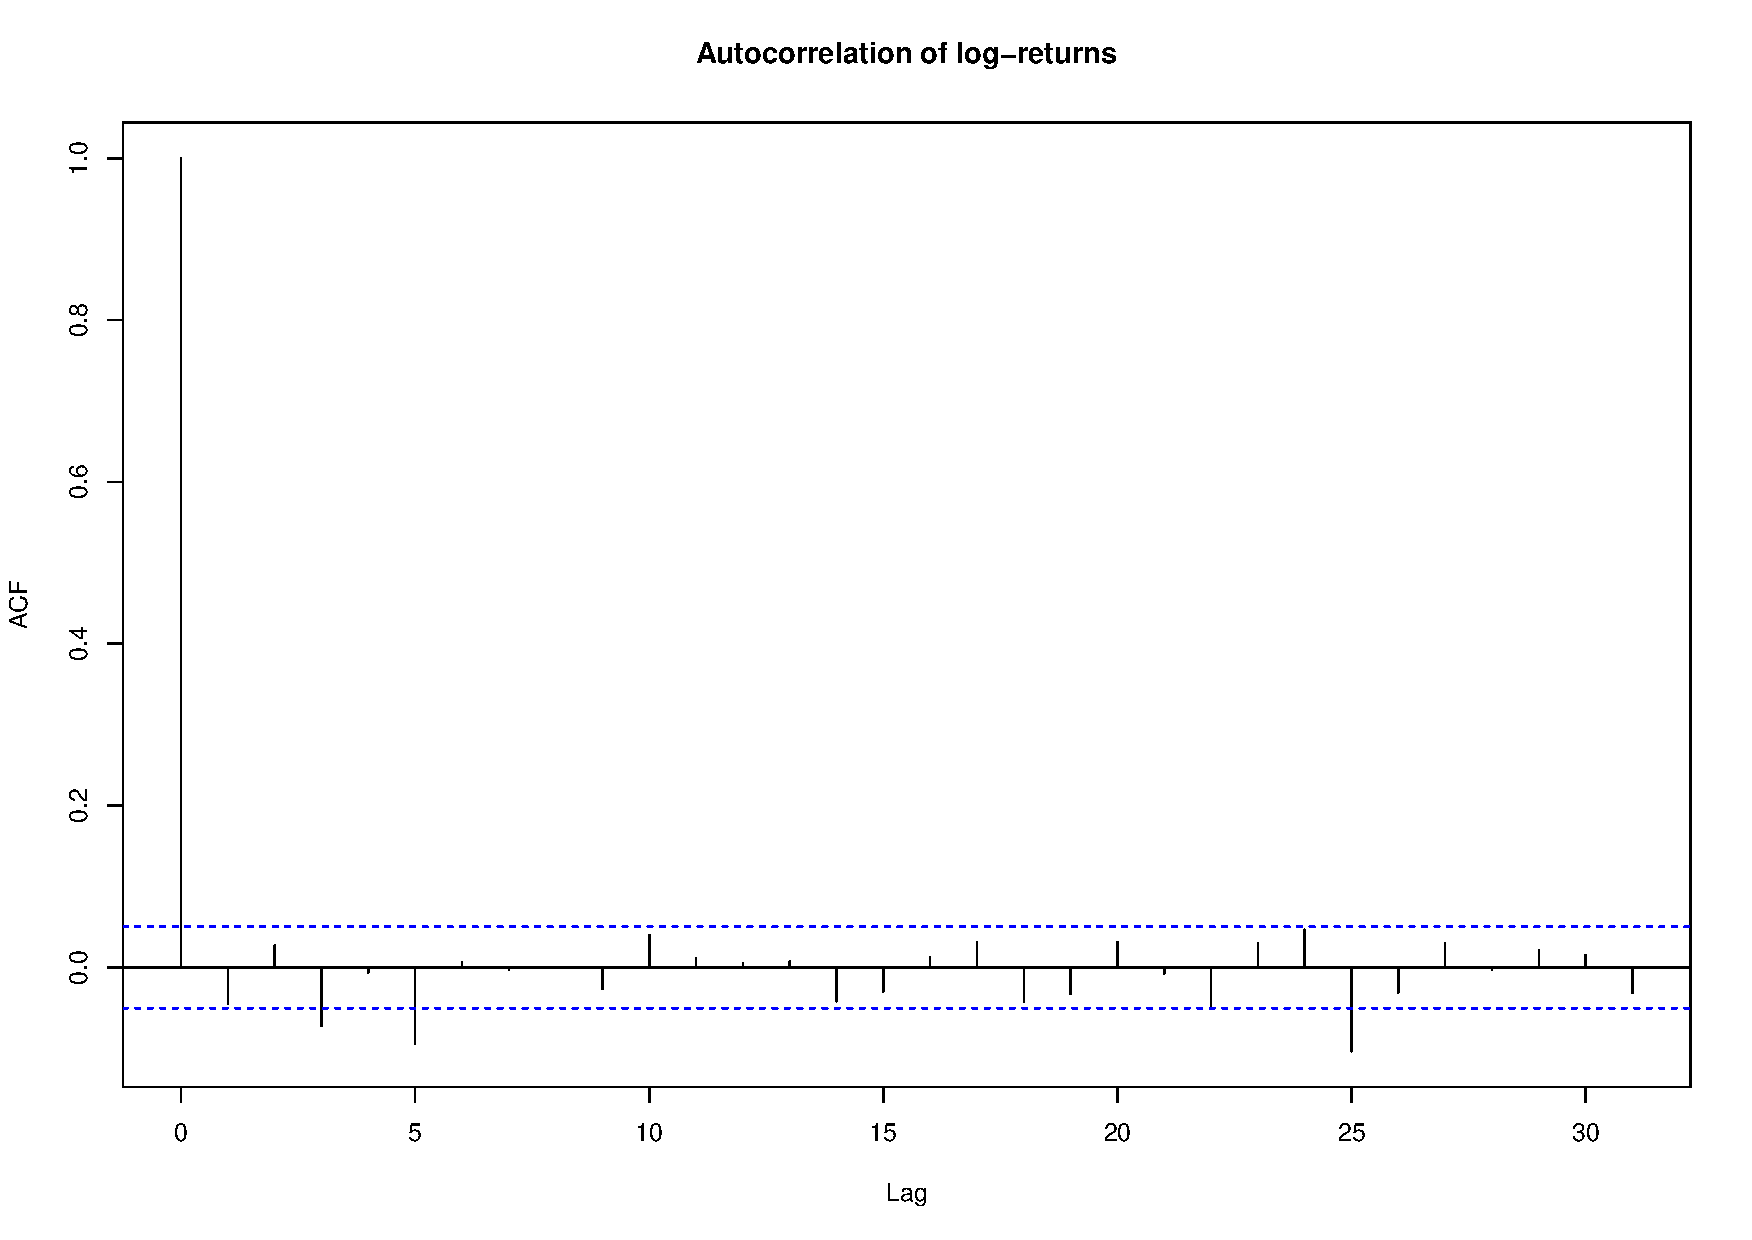
\includegraphics[width=.65\textwidth]
				{../Draft/img/finData/acfDailyLogRet}
				\caption{S\&P 500 ACF}
			\end{figure}
			
			\vspace{-.5cm}
			\begin{figure}
				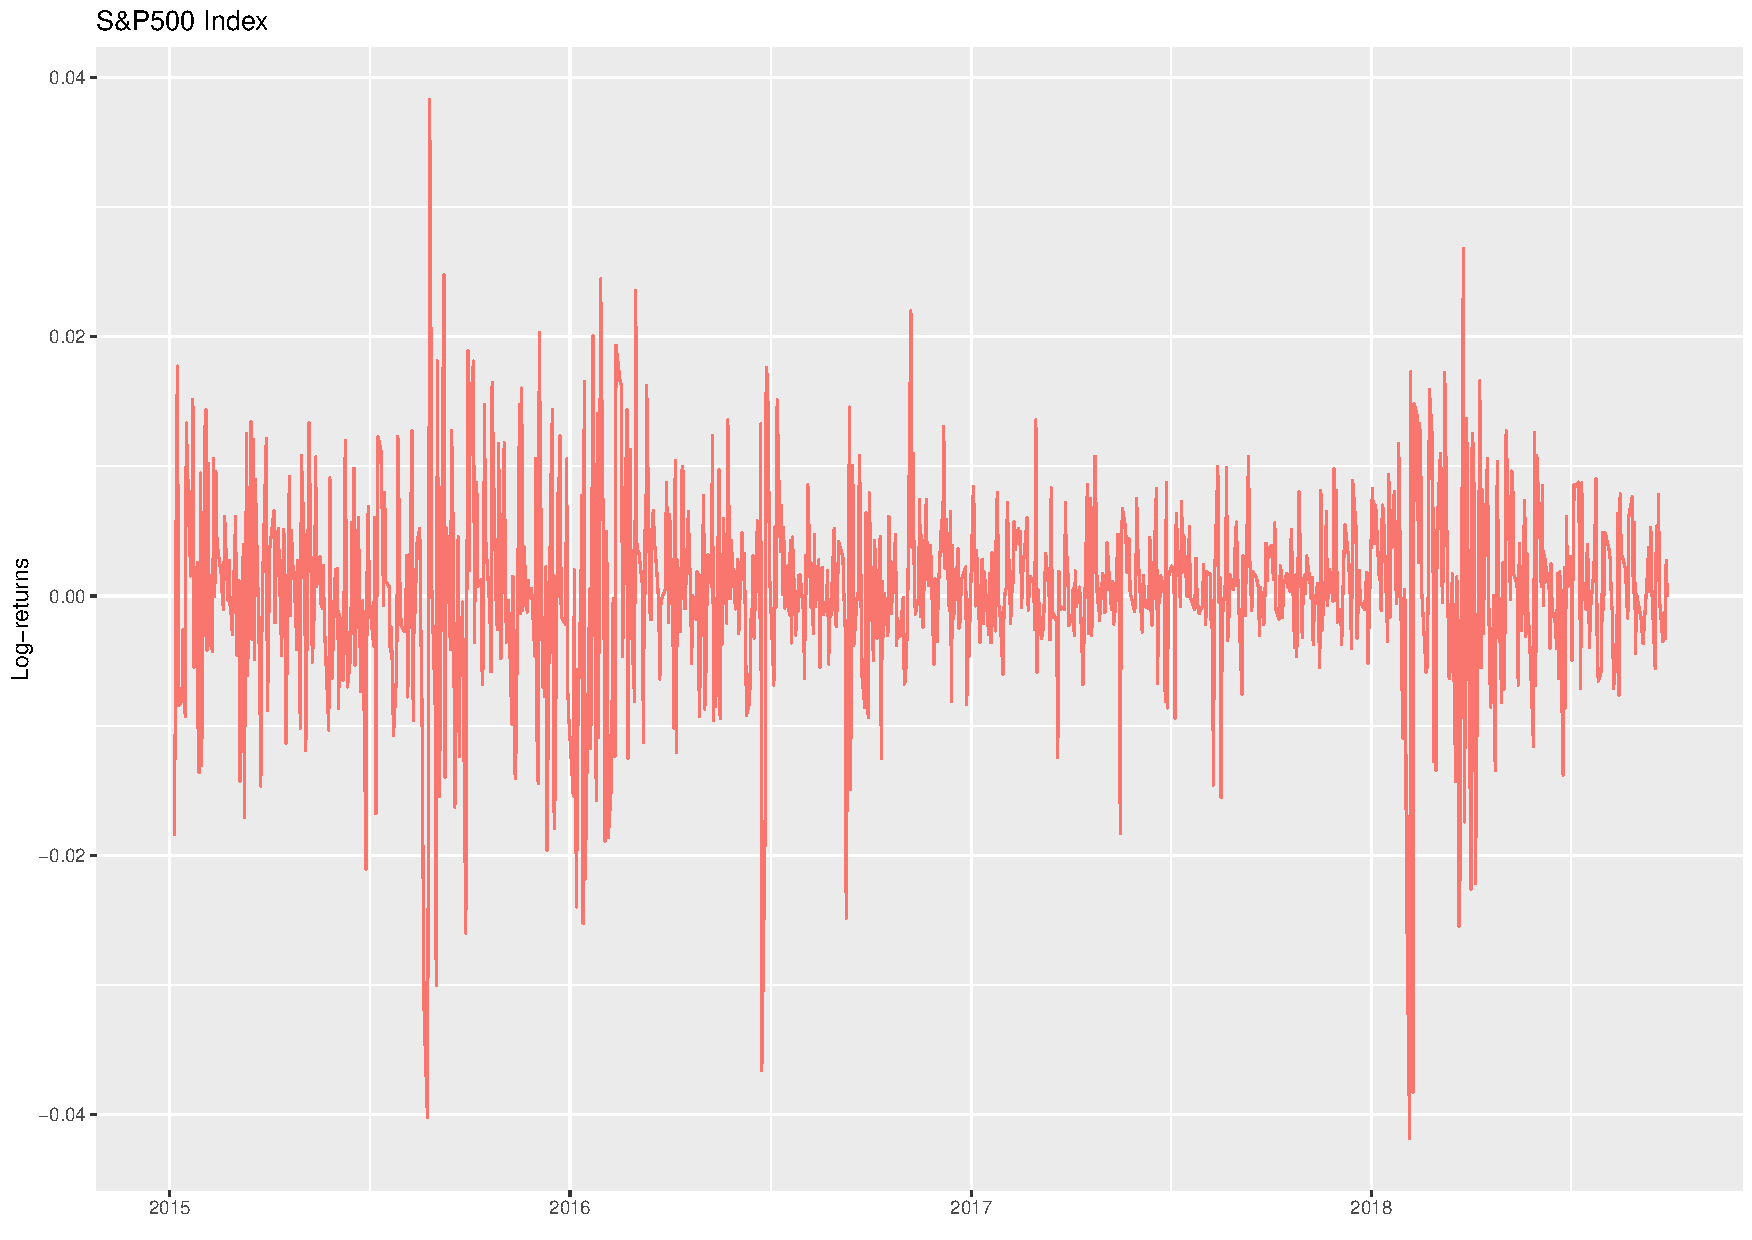
\includegraphics[width=.65\textwidth]
				{../Draft/img/finData/logReturns}
				\caption{S\&P 500 log-returns}
			\end{figure}
		\end{column}
		
		\begin{column}{.5\textwidth}
					
			\begin{figure}[hbtp]
				\begin{subfigure}{.5\textwidth}
					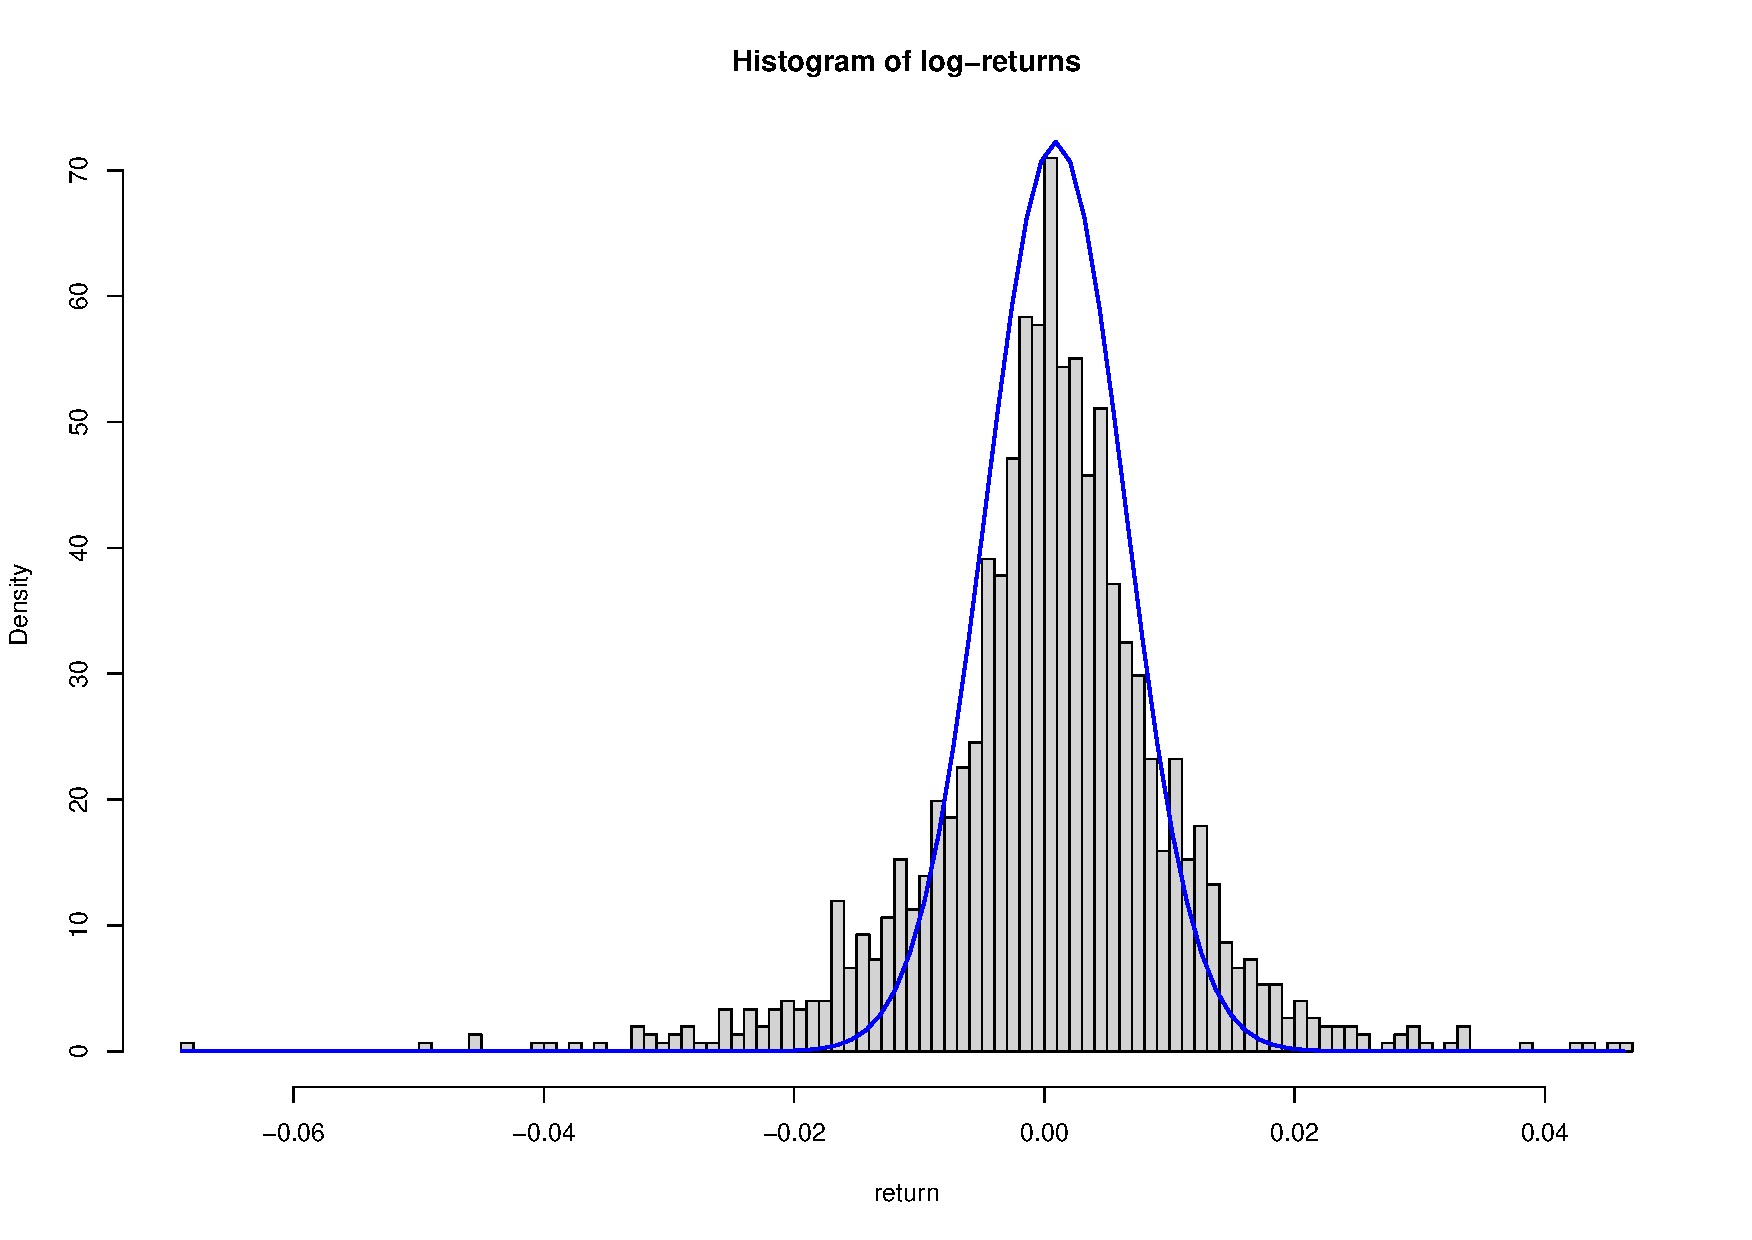
\includegraphics[scale=.11]
					{../Draft/img/finData/histDailyLogRet}
					\caption{Daily}
				\end{subfigure}%
				\begin{subfigure}{.5\textwidth}
					\centering
					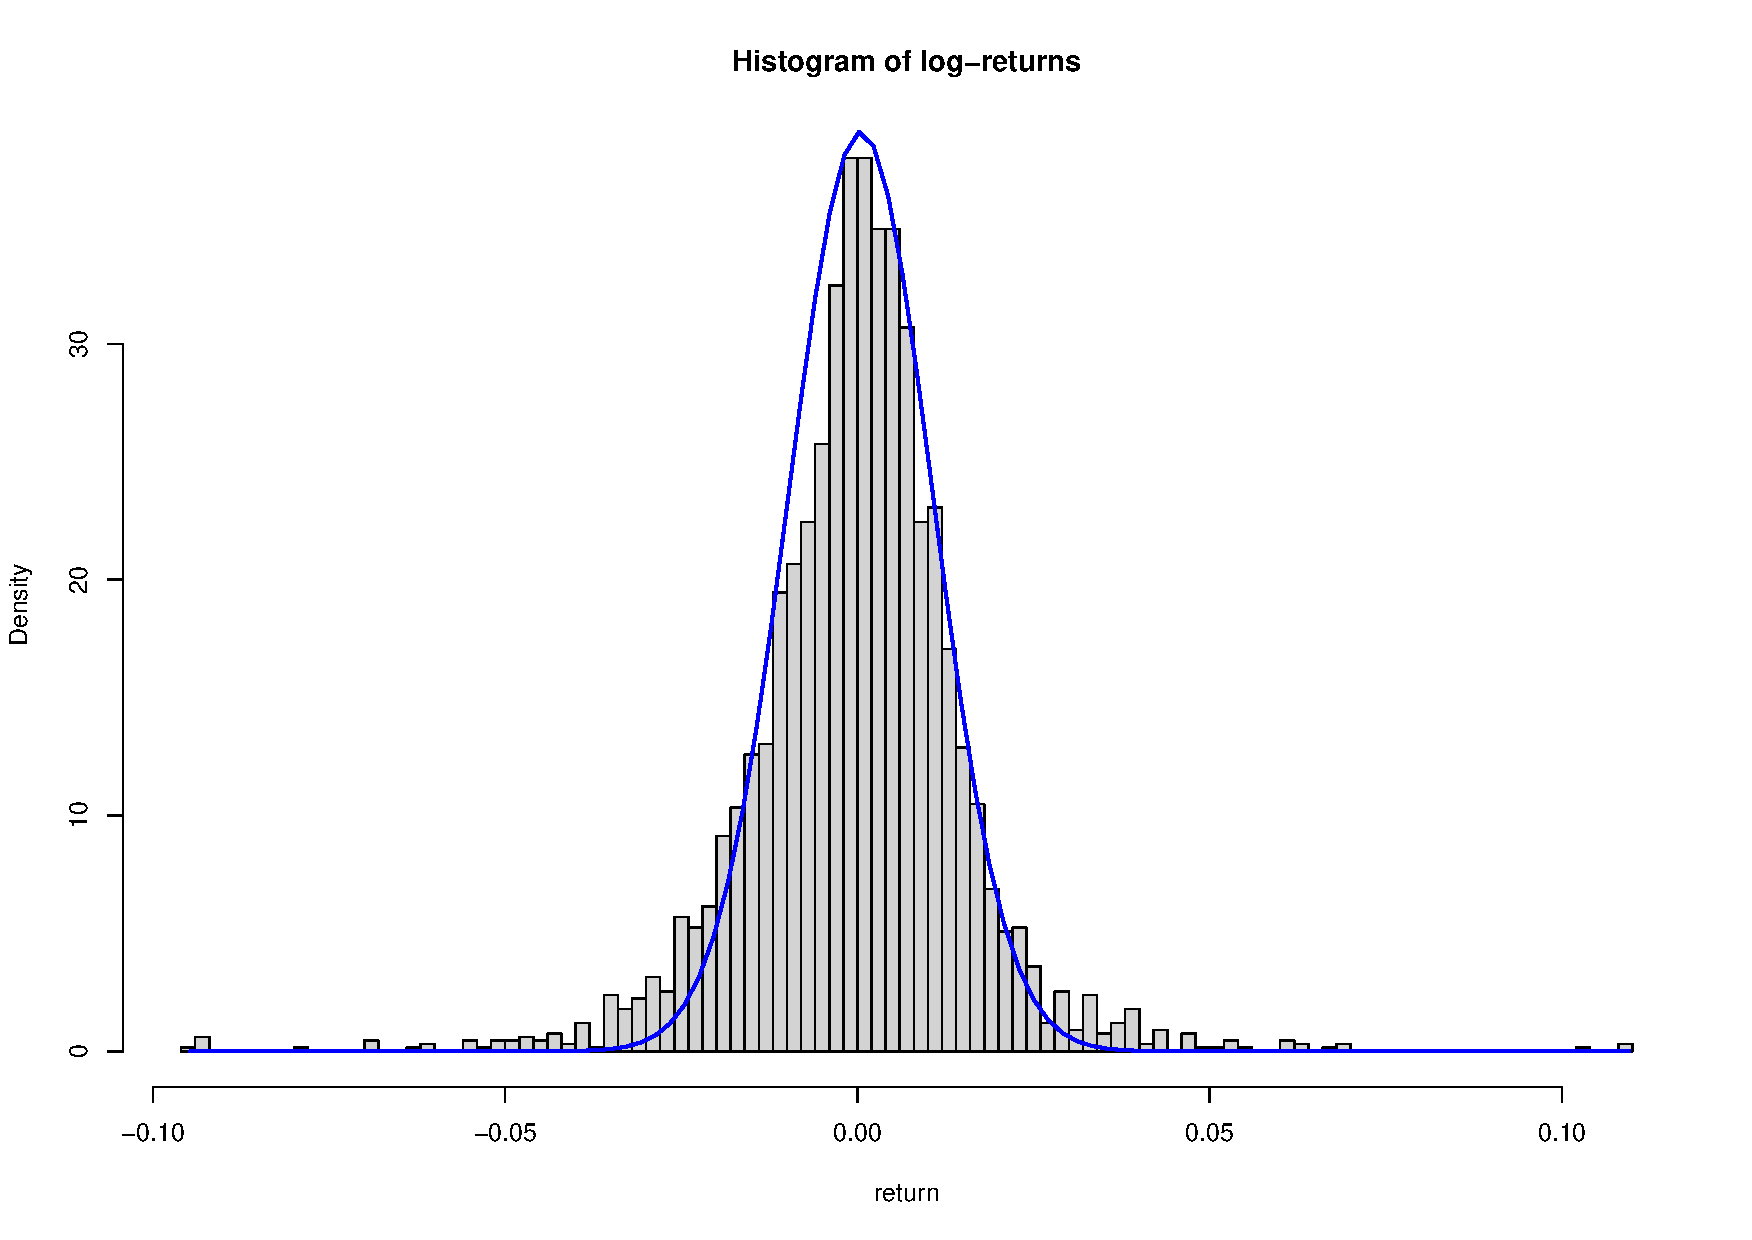
\includegraphics[scale=.11]
					{../Draft/img/finData/histWeeklyLogRet}
					\caption{Weekly}
				\end{subfigure}
				
				\begin{subfigure}{\textwidth}
					\centering
					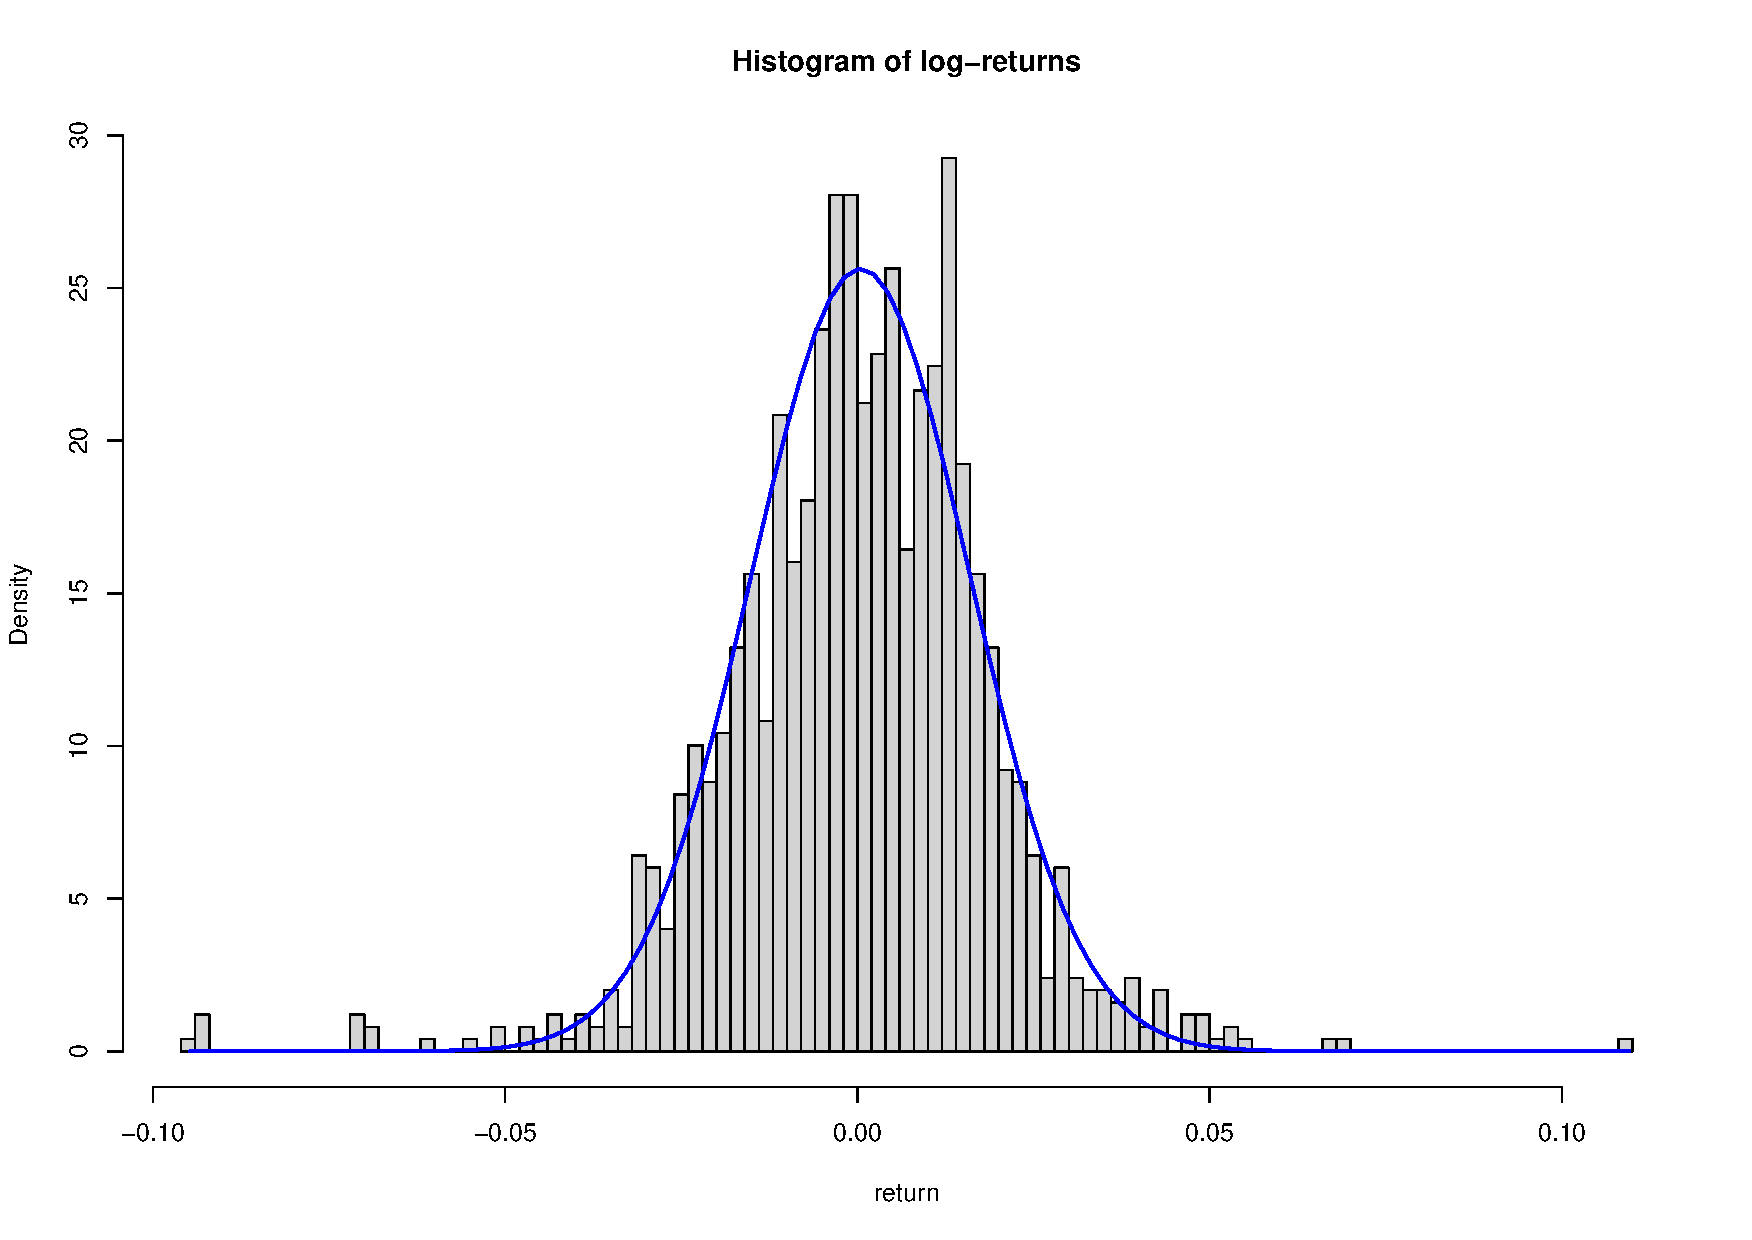
\includegraphics[scale=.11]
					{../Draft/img/finData/histMonthlyLogRet}
					\caption{Monthly}
				\end{subfigure}
				\caption{S\&P 500 log-returns histogram}

			\end{figure}
		\end{column}
	\end{columns}

\end{frame}

\begin{frame}{Side of a position}

\begin{block}{Long position}
A long position (or going long on some stock) is the most common way to 
invest. It just means that you buy an asset and you sell it at some point, 
expecting to earn a positive return.
\end{block}

\begin{block}{Short position}
If you short a stock, you first sell a stock that someone has lent you and 
then try to repurchase it at a lower price to return the stock to the lender. 
That way, if the \textbf{stock goes down in price}, you would \textbf{earn a 
profit} by selling high and buying low.
\end{block}

\begin{equation*}
	R_{t_1}^{\text{short}} = \frac{\text{profits}}{p_{t_0}} = \frac{p_{t_0} - 
	p_{t_1}}{p_{t_0}} = -R_{t_1}
\end{equation*}

\end{frame}

\begin{frame}{Financial Metrics}

\begin{block}{\centering{Sharpe Ratio}}
	\begin{center}
		$\text{SR} := \frac{\mathbb{E}[R_t - r_f]}{\sqrt{\text{Var}[R_t - 
		r_f]}}$, representing the reward per unit of risk.
	\end{center}
\end{block}

\begin{block}{\centering{Information Ratio}}
	\begin{center}
		$\text{IR} := \frac{\mathbb{E}[R_t - R_b]}{\sqrt{\text{Var}[R_t - 	
		R_b]}}$, where $R_b$ are the returns of a benchmark.
	\end{center}
\end{block}

\begin{block}{\centering{Drawdown}}
	\begin{center}
		It measures the relative drop from a historical peak.
		\vspace{-.15cm}
		\begin{equation*} 
			D(t) := \frac{\text{HWM}(t) - p_t}{\text{HWM}(t)} \text{, where } 
			\text{HWM}(t) = \max_{1 \leq \tau \leq t} p_{\tau}
		\end{equation*}
	\end{center}
\end{block}

\end{frame}

\begin{frame}{High Frequency Data}
	\vfill
	\begin{itemize}
		\item A \textbf{buy} (\textbf{sell}) order represents the will of a 
		trader to buy (sell) $m$ units of an asset at a price $p$.
	\end{itemize}

	\vfill
	Important concepts:
	\begin{itemize}
		\item \textbf{Bid price} ($b_t$): maximum price out of all the buy 
		orders at time $t$.
		
		\item \textbf{Ask price} ($a_t$): minimum price out of all the sell 
		orders at time $t$.
		
		\item \textbf{Mid price:} $m_t = \frac{a_t + b_t}{2}$
		
		%\item \textbf{Price:} ($p_t$) price of the last asset sold.
		
		\item \textbf{Volume:} ($v_t$) number of stocks exchanged.
		
		\item \textbf{Tick size:} smallest change in price a stock can move 
		(e.g. 0.001\$).
	\end{itemize}
	
	\vfill
	A \textbf{tick} is defined as $\{t, p_t, b_t, a_t, v_t \}$
	
	\vfill
\end{frame}

\begin{frame}{High Frequency Data}
	%\scalebox{0.5}{
	\begin{table}[htbp]
	\caption{Example of tick data (2013-01-02)}
	\centering
	\scalebox{0.8}{
	\begin{tabular}{ |C{2.5cm}|C{2cm}|C{2cm}|C{2cm}|C{2cm}| }
		\hline
		$t$ & $p_t$ & $b_t$ & $a_t$ & $v_t$\\
		\hline
		08:00:00 & 67.18 & 67.18 & 67.78 & 125\\
		08:12:56 & 67.70 & 67.19 & 67.70 & 125\\
		08:12:56 & 67.75 & 67.75 & 67.82 & 125\\
		08:47:15 & 67.91 & 67.21 & 67.93 & 150\\
		09:29:09 & 67.55 & 67.52 & 67.55 & 200\\
		09:29:09 & 67.56 & 67.51 & 67.57 & 200\\
		09:29:10 & 67.56 & 67.51 & 67.58 & 200\\
		09:29:10 & 67.58 & 67.51 & 67.57 & 100\\
		09:29:10 & 67.58 & 67.52 & 67.58 & 100\\
		09:29:11 & 67.57 & 67.52 & 67.58 & 200\\
		\hline
	\end{tabular}
	}
	\end{table}
	%}
\end{frame}

\section{Meta-labeling}
\begin{frame}{What is meta-labeling?}
	\begin{figure}[htbp]
		\centering
		\includegraphics[width=.8\textwidth]
		{"\homeCOne/img/metaLabelingDiagram2"}
\end{figure}
\end{frame}

\begin{frame}{Binary classification problem}
	\begin{block}{Primary model (M1)}
		It will predict the side of the investment. The labels will be noted 
		as $y_i^{\text{M1}} \in \{-1, 1\}$ and the predictions as 
		$\widehat{y}_i^{\text{M1}}$
	\end{block}
	\begin{block}{Secondary model (M2)}
		It will predict whether the primary model was right or not.\\
		The labels will be defined as:
		\scalebox{0.8}{		
		$
			y_i^{\text{M2}} = 
			\begin{cases}
				1 & \text{if } y_i^{\text{M1}} = \widehat{y}_i^{\text{M1}}\\
				0 & \text{otherwise}
			\end{cases}
		$
		}
		, while predictions will be noted as $\widehat{y}_i^{\text{M2}}$
	\end{block}
	\begin{block}{Meta-model}
		M1 + M2. It will \textbf{only} open a position, with the side 
		predicted by M1, when M2 determines that M1 is right.
	\end{block}
\end{frame}

\begin{frame}{Binary classification problem}
\begin{columns}

\begin{column}{.5\textwidth}
	%\vfill
	\textbf{\underline{Outcomes:}}\\
	\begin{itemize}
		\item \textbf{1} (Positive): Open a position
		\item \textbf{0} (Negative): Do not open a position
	\end{itemize}
	
	%\vfill
	\textbf{\underline{Metrics:}}\\
	\begin{itemize}
		\item \textbf{Recall} $= \frac{\text{TP}}{\text{TP} + \text{FN}}$
		\item \textbf{Precision} $= \frac{\text{TP}}{\text{TP} + \text{FP}}$
		\item \textbf{F1-Score} $= \frac{2}{\text{recall}^{-1} + 
		\text{precision}^{-1}}$
	\end{itemize}
	%\vfill
\end{column}
\begin{column}{.5\textwidth}
	\textbf{\underline{Possible predictions:}}\\
	\begin{itemize}
		\item \textbf{TP}: $y_i^{\text{M2}} = 1 = \widehat{y}_i^{\text{M2}}$
		\vspace{.2cm}
		
		\item \textbf{FP}: $y_i^{\text{M2}} = 0 \neq 
		\widehat{y}_i^{\text{M2}}$
		\vspace{.2cm}
		
		\item \textbf{TN}: $y_i^{\text{M2}} = 0 = \widehat{y}_i^{\text{M2}}$
		\vspace{.2cm}
		
		\item \textbf{FN}: $y_i^{\text{M2}} = 1 \neq 
		\widehat{y}_i^{\text{M2}}$
		\vspace{.2cm}
	\end{itemize}
\end{column}

\end{columns}
\end{frame}

\subsection{Toy Project}
\begin{frame}{Toy project}
	\framesubtitle{Features and labels}
	The main idea of this project was to determine how meta-labeling 
	works with synthetic data. In this case, 5 features have been 
	used: $\textbf{X}_1$, $\textbf{X}_2$, $\textbf{X}_3$, $\textbf{X}_4$ and 
	$\textbf{X}_5$.\\
	
	\begin{itemize}
		\item $\textbf{X}_{k, i} \sim N(\mu_i,\ \sigma^2)$
		
		\item $\omega_k = \textbf{sigmoid} \left( \alpha + 
		\sum_{i = 1}^{5} \textbf{X}_{k,i} \cdot \beta_i + \epsilon_k 
		\right)$ where $\epsilon_k \sim N(0,\ \sigma_{\epsilon}^2)$
	\end{itemize}
	
	\vspace{.2cm}
	
	The labels are defined as:

	\begin{equation*}
		y_k^{\text{M1}} =
	    \begin{cases}
	      -1 & \text{if}\ \omega_k < 0.5 \\
	      \hfill 1 & \text{otherwise} 
	    \end{cases}
	\end{equation*}
	
	In order to \textbf{simulate relative abundance and scarcity of data}, 
	models will use different features, e.g.:\\ 
	M1: $\textbf{X}_1$,$\textbf{X}_2$ \hspace{.25cm} M2: 
	$\widehat{y}^{\text{M1}}$, $\textbf{X}_3, \ldots , \textbf{X}_5$. 
	
\end{frame}

\begin{frame}{Results}
	\framesubtitle{Example}
	\vspace{-.3cm}
	To exemplify what meta-labeling does, the following models will be 
	analyzed:\\
	M1: $\textbf{X}_1,\textbf{X}_2$ \hspace{2cm} ($N_{\text{M1}} = 2$)\\
	M2: $\widehat{y}^{\text{M1}},\textbf{X}_3,\textbf{X}_4,\textbf{X}_5$
	\hspace{.57cm} ($N_{\text{M2}} = 4$)\\
	$\sigma_\epsilon = 0.3$
	\vfill
\begin{columns}
\begin{column}{.6\textwidth}
	\begin{figure}[htbp]
	\begin{subfigure}{.5\textwidth}
		\centering
		\scalebox{.45}{
		\renewcommand\arraystretch{1.5}
		\setlength\tabcolsep{0pt}
		\begin{tabular}{c >{\bfseries}r @{\hspace{0.7em}}c 
		@{\hspace{0.4em}}c @{\hspace{0.7em}}l}
		  \multirow{10}{*}{\parbox{1.1cm}{\bfseries\raggedleft Actual\\ 
		  value}} & 
		    & \multicolumn{2}{c}{\bfseries Prediction outcome} & \\
		  & & \bfseries 1 & \bfseries 0 & \bfseries Total \\
		  & 1 & \MyBox{TP}{143} & \MyBox{FN}{0} & 143 \\[2.4em]
		  & 0 & \MyBox{FP}{57} & \MyBox{TN}{0} & 57 \\
		  & Total & 200 & 0 &
		\end{tabular}}
		\caption{Primary Model}
		\label{toyProjectConfusionMatrixM1}
	\end{subfigure}%
	\begin{subfigure}{.5\textwidth}
		\centering
		\scalebox{0.45}{
		\renewcommand\arraystretch{1.5}
		\setlength\tabcolsep{0pt}
		\begin{tabular}{c >{\bfseries}r @{\hspace{0.7em}}c @{\hspace{0.4em}}c 
		@{\hspace{0.7em}}l}
		  \multirow{10}{*}{\parbox{1.1cm}{\bfseries\raggedleft Actual\\ 
		  value}} & & \multicolumn{2}{c}{\bfseries Prediction outcome} & \\
		  & & \bfseries 1 & \bfseries 0 & \bfseries Total \\
		  & 1 & \MyBox{TP}{136} & \MyBox{FN}{7} & 143 \\[2.4em]
		  & 0 & \MyBox{FP}{41} & \MyBox{TN}{16} & 57 \\
		  & Total & 177 & 23 &
		\end{tabular}}
		\caption{Meta-model}
		\label{toyProjectConfusionMatrixMM}
	\end{subfigure}
	
	\vspace{-.15cm}
	
	\caption{Confusion Matrices (Test)}
	%\label{toyProjectConfusionMatrices}
	\end{figure}
\end{column}

\begin{column}{.4\textwidth}
	\begin{figure}[htbp]
		\centering
		\includegraphics[scale=.15]{"\homeCOne/img/toyProjectMetrics"}
		\caption{Toy Project - Metrics of example (Test)}
		%\label{fig:toyProjectMetrics}
	\end{figure}
\end{column}
\end{columns}


\end{frame}

\begin{frame}{Results}
\framesubtitle{Precision}
\begin{figure}[htbp]
	\centering
	\begin{subfigure}{.5\textwidth}
	\centering
		\includegraphics[scale=.12]{"\homeCOne/img/toyProject/precisionN1"}
	  	\caption{$N_{\text{M1}} = 1$}
	  	\label{fig:precisionN1}
	\end{subfigure}%
	\begin{subfigure}{.5\textwidth}
	\centering
		\includegraphics[scale=.12]{"\homeCOne/img/toyProject/precisionN2"}
		\caption{$N_{\text{M1}} = 2$}
		\label{fig:precisionN2}
	\end{subfigure}

	%\vspace{.5cm}

	\begin{subfigure}{.5\textwidth}
	\centering
		\includegraphics[scale=.12]{"\homeCOne/img/toyProject/precisionN3"}
		\caption{$N_{\text{M1}} = 3$}
		\label{fig:precisionN3}
	\end{subfigure}%
	\begin{subfigure}{.5\textwidth}
	\centering
		\includegraphics[scale=.12]{"\homeCOne/img/toyProject/precisionN4"}
		\caption{$N_{\text{M1}} = 4$}
		\label{fig:precisionN4}
	\end{subfigure}
	\vspace{-.3cm}
	\caption{Precision (Test)}
\end{figure}

\end{frame}

\begin{frame}{Results}
\framesubtitle{Recall}
\begin{figure}[htbp]
	\centering
	\begin{subfigure}{.5\textwidth}
	\centering
		\includegraphics[scale=.12]{"\homeCOne/img/toyProject/recallN1"}
	  	\caption{$N_{\text{M1}} = 1$}
	  	\label{fig:precisionN1}
	\end{subfigure}%
	\begin{subfigure}{.5\textwidth}
	\centering
		\includegraphics[scale=.12]{"\homeCOne/img/toyProject/recallN2"}
		\caption{$N_{\text{M1}} = 2$}
	\end{subfigure}

	%\vspace{.5cm}

	\begin{subfigure}{.5\textwidth}
	\centering
		\includegraphics[scale=.12]{"\homeCOne/img/toyProject/recallN3"}
		\caption{$N_{\text{M1}} = 3$}
	\end{subfigure}%
	\begin{subfigure}{.5\textwidth}
	\centering
		\includegraphics[scale=.12]{"\homeCOne/img/toyProject/recallN4"}
		\caption{$N_{\text{M1}} = 4$}
	\end{subfigure}
	%\vspace{-.1cm}
	\caption{Recall (Test)}
\end{figure}

\end{frame}

\begin{frame}{Results}
\framesubtitle{F1-Score}
\begin{figure}[htbp]
	\centering
	\begin{subfigure}{.5\textwidth}
	\centering
		\includegraphics[scale=.12]{"\homeCOne/img/toyProject/F1ScoreN1"}
	  	\caption{$N_{\text{M1}} = 1$}
	\end{subfigure}%
	\begin{subfigure}{.5\textwidth}
	\centering
		\includegraphics[scale=.12]{"\homeCOne/img/toyProject/F1ScoreN2"}
		\caption{$N_{\text{M1}} = 2$}
	\end{subfigure}

	\vspace{.2cm}

	\begin{subfigure}{.5\textwidth}
	\centering
		\includegraphics[scale=.12]{"\homeCOne/img/toyProject/F1ScoreN3"}
		\caption{$N_{\text{M1}} = 3$}
	\end{subfigure}%
	\begin{subfigure}{.5\textwidth}
	\centering
		\includegraphics[scale=.12]{"\homeCOne/img/toyProject/F1ScoreN4"}
		\caption{$N_{\text{M1}} = 4$}
	\end{subfigure}
	%\vspace{-.3cm}
	\caption{F1-Score (Test)}
\end{figure}

\end{frame}

\subsection{Financial Project}
\begin{frame}{Data}
\begin{figure}[htbp]
	\centering
	\includegraphics[scale=.2]{"\homeCOne/img/removalOutliersGMVP"}
	\caption{Imputed log-price time series of the S\&P 500 GMVP}
	\label{fig:removalOutlierGMVP}
\end{figure}

\vspace{-.4cm}

\begin{figure}[htbp]
	\centering
	\includegraphics[scale=.05]{"\homeCOne/img/dataDivision"}
	%\caption{Data Division}
	%\label{fig:dataDivision}
\end{figure}

\end{frame}

\begin{frame}{Triple barrier method}
\framesubtitle{Symmetric barriers}
\begin{columns}
\begin{column}{.6\textwidth}
\begin{figure}
	\centering
	\includegraphics[width=.95\textwidth]
	{"\homeCOne/img/tripleBarrierSymmetric"}
	\caption{Symmetric barriers}
\end{figure}
\end{column}
\begin{column}{.4\textwidth}
	\begin{itemize}
		\item \textbf{Upper horizontal barrier:} $p_{t_{i,0}} (1 + \text{pt} 
		\cdot \sigma_{t_{i,0}})$
		
		\item \textbf{Lower horizontal barrier:} $p_{t_{i,0}} (1 - \text{sl} 
		\cdot \sigma_{t_{i,0}})$	
	
	\vspace{.2cm}
	\hspace{-.5cm} where pt = sl = 2.
	\vspace{.2cm}
		
		\item \textbf{Vertical barrier:} 10 days.
	\end{itemize}

	\begin{center}
	\scalebox{0.85}{
	$
		y_i =
	    \begin{cases}
	      1 & \text{if } R_i > 0 \\
	      0 & \text{otherwise}
	    \end{cases}
	$
	}
	, where
	\scalebox{0.85}{
	$
		R_i = (1 - \text{tc})^2 \cdot \left( \frac{p_{t_{i,1}}}{p_{t_{i,0}}} 
		- 1 \right)
	$	
	}
	\end{center}
\end{column}
\end{columns}

\end{frame}

\begin{frame}{Triple barrier method}
\framesubtitle{Notation when the side is known}
\begin{itemize}
	\item \textbf{Upper horizontal barrier:} $p_{t_{i,0}} (1 + 
	\delta_{+, t_{i,0}})$, where\\
	
	\vspace{.2cm}
	\scalebox{0.85}{	
	$
	\delta_{+, t_{i,0}} =
    \begin{cases}
      \text{pt} \cdot \sigma_{t_{i,0}} & \text{if}\ 
      \widehat{y}^{\text{M1}}_{i} = 1 \\
      \min(0.5\%,\ \frac{1}{2} \cdot \text{pt} \cdot \sigma_{t_{i,0}}) & 
      \text{otherwise}
    \end{cases}
	$
	}
	\vspace{.2cm}
	
	\item \textbf{Lower horizontal barrier:} $p_{t_{i,0}} (1 - 
	\delta_{-, t_{i,0}})$, where\\
	
	\vspace{.2cm}
	\scalebox{0.85}{
	$
	\delta_{-, t_{i,0}} =
    \begin{cases}
      \text{sl} \cdot \sigma_{t_{i,0}} & \text{if}\ 
      \widehat{y}^{\text{M1}}_{i} = -1 \\
      \min(0.5\%,\ \frac{1}{2} \cdot \text{sl} \cdot \sigma_{t_{i,0}}) & 	
      \text{otherwise}
    \end{cases}
	$    
    }
    \vspace{.2cm}
	
	\item Predicted \textbf{Side of the trade} starting on 
	$\boldsymbol{t_{i,0}}$: $\widehat{y}_i^{\text{M1}}$
\end{itemize}

\end{frame}

\begin{frame}{Triple barrier method}
\framesubtitle{Adaptation when the side is known}
\begin{columns}
\begin{column}{.6\textwidth}
\begin{figure}
	\centering
	\includegraphics[width=.95\textwidth]
	{"\homeCOne/img/tripleBarrierSide"}
	\caption{Triple Barrier Labeling when $y_i^{\text{M1}} = -1$}
	%\label{fig:tripleBarrierSymmetric}
\end{figure}
\end{column}
\begin{column}{.4\textwidth}
	\begin{center}
	\scalebox{0.85}{
	$
		y^{\text{M2}}_i =
	    \begin{cases}
	      1 & \text{if}\ R_i > 0 \\
	      0 & \text{otherwise}
	    \end{cases}
	$
	}
	\end{center}
	Where
	\begin{center}
	\scalebox{0.85}{
	$
		R_i = (1 - \text{tc})^2 \cdot \left( \frac{p_{t_{i,1}}}{p_{t_{i,0}}} 
		- 1 \right) \cdot \widehat{y}^{\text{M1}}_{i}
	$	
	}
	\end{center}
\end{column}
\end{columns}

\end{frame}

\begin{frame}{Primary models}
\begin{columns}
\begin{column}{.45\textwidth}
	\begin{block}{\centering{MA based}}
	Deterministic moving average (MA) crossovers:\\
	\begin{itemize}
		\item \textbf{Entry points:} CUSUM filter
		
		\vspace{.2cm}
		\item \textbf{Labels:}
		
		\vspace{.2cm}
		\scalebox{0.6}{
		$
			y_{i}^{\text{M1}} = 
			\begin{cases}
			\hfill 1 & \text{if}\ 
			R_i = (1 - \text{tc})^2 \left( \frac{p_{t_{i,1}}}{p_{t_{i,0}}} -1 
			\right) > 0\\
			\hfill -1 & \text{otherwise}	
			\end{cases}
		$
		}
		
		\vspace{.2cm}
		\item \textbf{Predictions:}
		
		\vspace{.2cm}
		\scalebox{0.6}{
		$
			\widehat{y}_i^{\text{M1}} =
			\begin{cases}
				\hfill 1  & \text{if}\ \text{MA}_i < p_{t_{i,0}}\\
				\hfill -1 & \text{if}\ \text{MA}_i \geq p_{t_{i,0}}
			\end{cases}
		$
		}
	\end{itemize}
	\end{block}
\end{column}

\begin{column}{.45\textwidth}
	\begin{block}{\centering{ML based}}
	\begin{itemize}
		\item \textbf{Features:}
		\scalebox{0.5}{ 
		$\log \left( \frac{\text{MA}_t}{p_t}	\right)$, 
		$\frac{\text{CUSUM}_{+,\ t}}{\sigma_t}$, 
		$\frac{\text{CUSUM}_{-,\ t}}{\sigma_t}$, 
		$\textbf{Reset}_{\text{CUSUM}_{+},t}$,
		}
		\scalebox{0.5}{		
		$\textbf{Reset}_{\text{CUSUM}_{-,t}}$ and 
		$\text{EWMSD}_t$
		}
		
		\vspace{.2cm}
		\item \textbf{Labels:}
		\scalebox{0.6}{
		$
			y_{i}^{\text{M1}} = 
			\begin{cases}
			\hfill 1 & \text{if}\ 
			R_i > 0\\
			\hfill -1 & \text{otherwise}	
			\end{cases}
		$
		}
		
		\vspace{.2cm}		
		\item \textbf{Predictions:} 
		\scalebox{0.6}{$\widehat{y}_i^{\text{M1}}$}
	\end{itemize}
	\end{block}
\end{column}
\end{columns}

\end{frame}

\begin{frame}{Secondary models}
\begin{columns}
\begin{column}{.45\textwidth}
	\begin{block}{\centering{MA based}}
	It will use a random forest with the following \textbf{features}:
	
	\vspace{.2cm}	
	\scalebox{0.5}{
	$\log \left( \frac{\text{MA}_{i}}{p_{t_{i,0}}} \right)$,
	$r_{t_{i,0}}$,
	$\underline{r_{t_{i,0}}} := \left( \prod_{k=0}^{4} 
	(1 + r_{t_{i,0}-k}) 	\right) - 1$, 
	$\widehat{y}_{i}^{\text{M1}}$, 
	$\text{RSI}_{t_{i,0},\ 9}$, 
	}
	
	\scalebox{0.5}{	
	$\text{RSI}_{t_{i,0},\ 14},\ 
	\text{RSI}_{t_{i,0},\ 25}$,
	$\tilde{\sigma}_{t_{i,0}}$,
	$\sigma_{t_{i,0},\ 9},\ \sigma_{t_{i,0},\ 14},\ \sigma_{t_{i,0},\ 25}$,
	$\text{ACF}_{t_{i,0},\ 1}$
	}
	\scalebox{0.5}{	
	and $\text{ACF}_{t_{i,0},\ 5}$
	}
	
	\vspace{.2cm}
	With \textbf{labels}:
	
	\vspace{.2cm}
	%\begin{center}
	\scalebox{0.6}{
	$
	y^{\text{M2}}_i =
	\begin{cases}
	1 & \text{if}\ y^{\text{M1}}_i = \widehat{y}^{\text{M1}}_i\\
	0 & \text{otherwise}
	\end{cases}
	$	
	}
	%\end{center}

	\end{block}
\end{column}

\begin{column}{.45\textwidth}
	\begin{block}{\centering{ML based}}
	Then only difference with the MA based M2 is the underlying Machine 
	Learning model.\\
	
	\vspace{.2cm}
	
	The 	ML based M2 will use a neural network with a hidden layer (25 fully 
	connected units - Leaky ReLU) and an output layer (Sigmoid).

	\end{block}
\end{column}
\end{columns}

\end{frame}

\begin{frame}{Hyper-parameter tuning}

\end{frame}

\begin{frame}{Results}

\end{frame}

\begin{frame}{Coin flip correction}

\end{frame}

\section{Fractional differentiation}
\begin{frame}{This}
	Rr
\end{frame}

\subsection{Toy Project}
\begin{frame}{This}
	This
\end{frame}

\subsection{Financial Project}
\begin{frame}{This}
	This
\end{frame}


\section{Data parsing as bars}
\begin{frame}{This}
	HFT
\end{frame}

\section{}
\begin{frame}{Conclusions and future work}

\end{frame}

\section{}
\begin{frame}
	\Large
	\begin{center}
		\textbf{Thank you for your attention}
		% Thank you for your attention	
	\end{center}

\end{frame}

\end{document}
